\section{main.cpp File Reference}
\label{main_8cpp}\index{main.cpp@{main.cpp}}


{\tt \#include \char`\"{}hdass08.h\char`\"{}}\par
{\tt \#include \char`\"{}kstartuplogo.h\char`\"{}}\par
{\tt \#include \char`\"{}global\_\-define.h\char`\"{}}\par
{\tt \#include $<$kapplication.h$>$}\par
{\tt \#include $<$kaboutdata.h$>$}\par
{\tt \#include $<$kcmdlineargs.h$>$}\par
{\tt \#include $<$klocale.h$>$}\par


Include dependency graph for main.cpp:\begin{figure}[H]
\begin{center}
\leavevmode
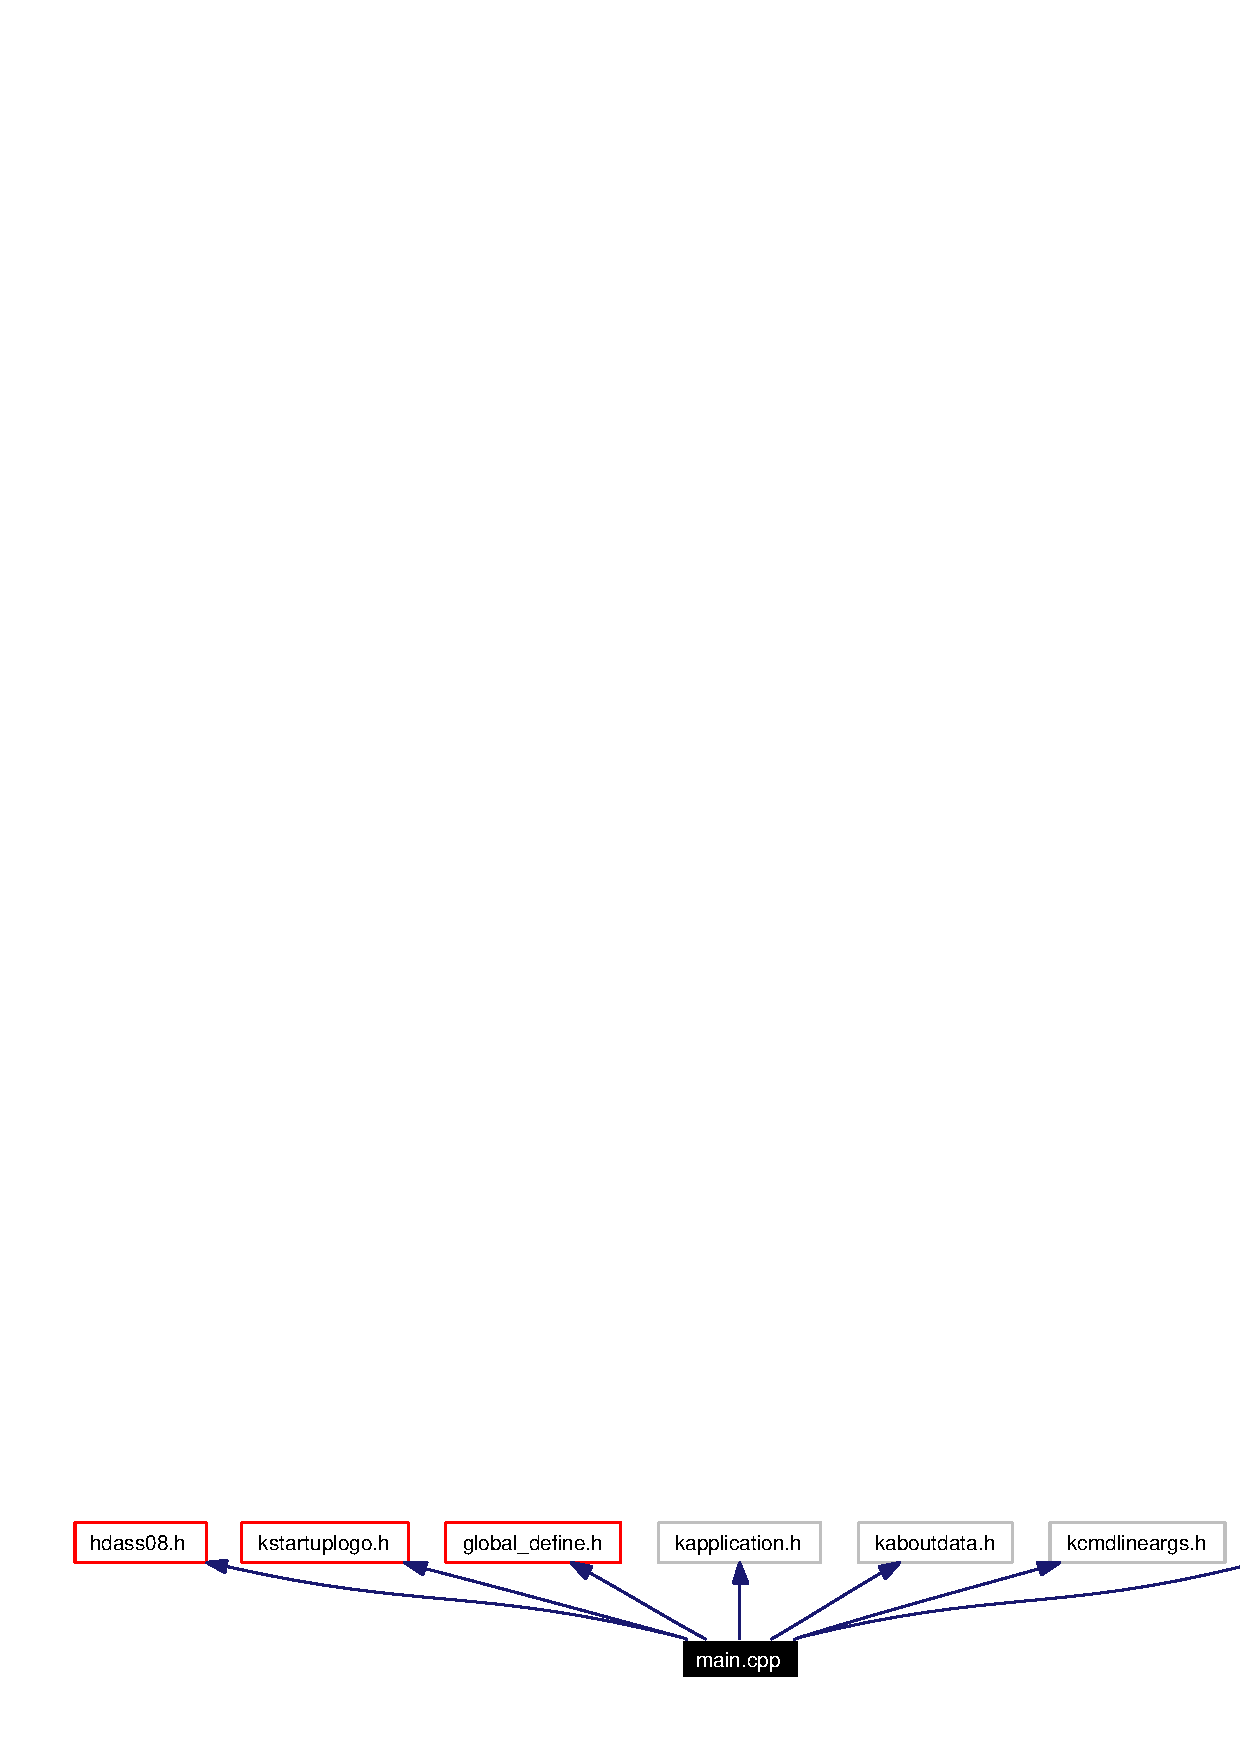
\includegraphics[width=331pt]{main_8cpp__incl}
\end{center}
\end{figure}
\subsection*{Functions}
\begin{CompactItemize}
\item 
void {\bf HDASS\_\-INIT} ()
\item 
int {\bf main} (int argc, char $\ast$$\ast$argv)
\end{CompactItemize}
\subsection*{Variables}
\begin{CompactItemize}
\item 
int {\bf int\-HDASS\_\-FUNCTION\_\-STATE}
\item 
{\bf HDASSGlobal\-Setting} {\bf Global\-Setting}
\item 
const char {\bf description} [$\,$]
\item 
const char {\bf version} [$\,$] = \char`\"{}0.1\char`\"{}
\item 
KCmd\-Line\-Options {\bf options} [$\,$]
\end{CompactItemize}


\subsection{Function Documentation}
\index{main.cpp@{main.cpp}!HDASS_INIT@{HDASS\_\-INIT}}
\index{HDASS_INIT@{HDASS\_\-INIT}!main.cpp@{main.cpp}}
\subsubsection{\setlength{\rightskip}{0pt plus 5cm}void HDASS\_\-INIT ()}\label{main_8cpp_a5}




Definition at line 46 of file main.cpp.

References em\_\-internet.

Referenced by main().



\footnotesize\begin{verbatim}47 {
48   intHDASS_FUNCTION_STATE=em_internet;
49 }
\end{verbatim}\normalsize 
\index{main.cpp@{main.cpp}!main@{main}}
\index{main@{main}!main.cpp@{main.cpp}}
\subsubsection{\setlength{\rightskip}{0pt plus 5cm}int main (int {\em argc}, char $\ast$$\ast$ {\em argv})}\label{main_8cpp_a6}




Definition at line 50 of file main.cpp.

References description, HDASS\_\-INIT(), main\-Win, options, and version.



\footnotesize\begin{verbatim}51 {
52     KAboutData about("hdass08", I18N_NOOP("HDASS08"), version, description,
53                      KAboutData::License_GPL, "(C) 2005 sonicat", 0, 0, "is87098@cis.nctu.edu.tw");
54     about.addAuthor( "sonicat", 0, "is87098@cis.nctu.edu.tw" );
55     KCmdLineArgs::init(argc, argv, &about);
56     KCmdLineArgs::addCmdLineOptions( options );
57     KApplication app;
58     HDASS08 *mainWin = 0;
59 
60     if (app.isRestored())
61     {
62         RESTORE(HDASS08);
63     }
64     else
65     {
66         // no session.. just start up normally
67         KCmdLineArgs *args = KCmdLineArgs::parsedArgs();
68 
69         //DAVID HDASS Logo Init Here//
70         KStartupLogo* HDASS_logo=NULL;
71         HDASS_logo = new KStartupLogo();
72         HDASS_logo->show();
73         
74         //Init All HDASS Setting 
75         HDASS_INIT();
76         
77         mainWin = new HDASS08();
78         mainWin->setGeometry(0,0,800,600);
79         
80         //DAVID this connection let HDASS_logo to trigger the mainWin
81         QObject::connect(HDASS_logo,SIGNAL(signalTriggerMainWidget()),mainWin,SLOT(slotShow()));
82         
83  
84         //mainWin->show();
85          
86         args->clear();
87     }
88 
89     // mainWin has WDestructiveClose flag by default, so it will delete itself.
90     return app.exec();
91 }
\end{verbatim}\normalsize 


Here is the call graph for this function:\begin{figure}[H]
\begin{center}
\leavevmode

\includegraphics[width=93pt]{main_8cpp_a6_cgraph}
\end{center}
\end{figure}


\subsection{Variable Documentation}
\index{main.cpp@{main.cpp}!description@{description}}
\index{description@{description}!main.cpp@{main.cpp}}
\subsubsection{\setlength{\rightskip}{0pt plus 5cm}const char {\bf description}[$\,$]\hspace{0.3cm}{\tt  [static]}}\label{main_8cpp_a2}


{\bf Initial value:}

\footnotesize\begin{verbatim}
    I18N_NOOP("A KDE KPart Application")
\end{verbatim}\normalsize 


Definition at line 35 of file main.cpp.

Referenced by main().\index{main.cpp@{main.cpp}!GlobalSetting@{GlobalSetting}}
\index{GlobalSetting@{GlobalSetting}!main.cpp@{main.cpp}}
\subsubsection{\setlength{\rightskip}{0pt plus 5cm}{\bf HDASSGlobal\-Setting} {\bf Global\-Setting}}\label{main_8cpp_a1}




Definition at line 34 of file main.cpp.

Referenced by Sub\-Bar\-Album\-Clock::Change\-Button\-Graphic(), hdassplaylist::Save\-List(), Function\-Bar::slot\-Change\-Function\-Sub\-Bar(), Sub\-Bar\-Album\-Clock::slot\-Change\-Mode(), Function\_\-Control\_\-Area::slot\-Image\-Detial(), Function\_\-Control\_\-Area::slot\-Process\-Change\-Func(), Function\_\-Control\_\-Area::slot\-Show\-Image\-Detial(), Display\-Area::x\-Setup(), Function\_\-Control\_\-Area::x\-Setup(), Function\-Bar::x\-Setup(), and hdassplaylist::x\-Setup().\index{main.cpp@{main.cpp}!intHDASS_FUNCTION_STATE@{intHDASS\_\-FUNCTION\_\-STATE}}
\index{intHDASS_FUNCTION_STATE@{intHDASS\_\-FUNCTION\_\-STATE}!main.cpp@{main.cpp}}
\subsubsection{\setlength{\rightskip}{0pt plus 5cm}int {\bf int\-HDASS\_\-FUNCTION\_\-STATE}}\label{main_8cpp_a0}




Definition at line 33 of file main.cpp.\index{main.cpp@{main.cpp}!options@{options}}
\index{options@{options}!main.cpp@{main.cpp}}
\subsubsection{\setlength{\rightskip}{0pt plus 5cm}KCmd\-Line\-Options {\bf options}[$\,$]\hspace{0.3cm}{\tt  [static]}}\label{main_8cpp_a4}


{\bf Initial value:}

\footnotesize\begin{verbatim}
{

    KCmdLineLastOption
}
\end{verbatim}\normalsize 


Definition at line 40 of file main.cpp.

Referenced by main().\index{main.cpp@{main.cpp}!version@{version}}
\index{version@{version}!main.cpp@{main.cpp}}
\subsubsection{\setlength{\rightskip}{0pt plus 5cm}const char {\bf version}[$\,$] = \char`\"{}0.1\char`\"{}\hspace{0.3cm}{\tt  [static]}}\label{main_8cpp_a3}




Definition at line 38 of file main.cpp.

Referenced by main().